\documentclass{IEEEtran}

\usepackage{cite}
\usepackage{amsmath}
\usepackage{amssymb}
\usepackage{url}
\usepackage{graphicx}
\usepackage{booktabs}
\usepackage{microtype}
\usepackage[table]{xcolor}
\usepackage{tikz}
\usetikzlibrary{positioning,arrows.meta,fit,backgrounds}
\usepackage[hidelinks]{hyperref}

\definecolor{PhaseGreen}{RGB}{45,176,150}
\definecolor{PhaseBlue}{RGB}{52,190,255}
\definecolor{PhasePurple}{RGB}{126,87,194}
\definecolor{PhaseOrange}{RGB}{245,166,35}
\definecolor{DeepNavy}{RGB}{11,26,51}

\title{A Fairness-Aware Sequential Routing Framework for Clinical Diagnostic Workflows and Quantum Routing\\[0.3em]
{\large\textit{Comparing Multi-Armed, Contextual, and Informative Bandit Methods}}}

\author{%
\begin{minipage}{0.48\textwidth}
\begin{center}
{\bf Piter Z. Garcia}\\
\begin{small}
MS Data Science / Decision-Making \& Algorithmic Fairness\\
Rochester Institute of Technology (RIT)\\
{\it pizg8794@g.rit.edu}
\end{small}
\end{center}
\end{minipage}
\hfill
\begin{minipage}{0.48\textwidth}
\begin{center}
{\bf Dr. Daniel Krutz, Travis Desell}\\
\begin{small}
Department of Software Engineering, Data Science\\
RIT Research Advisors\\
{\it dxkvse@g.rit.edu, tjdvse@g.rit.edu}
\end{small}
\end{center}
\end{minipage}%
}

\begin{document}
\maketitle
\vspace{-0.8em}

\section{Approach}

\subsection*{What is the approach to the work?}
This project proposes one fairness-aware sequential routing framework for two settings that at first look unrelated but share the same core problem. In the clinical setting, the system routes patients, tests, and escalation effort through a diagnostic pathway. In the quantum setting, the system routes entanglement and scarce network resources through candidate paths under probabilistic network conditions. The true common ground is therefore routing under scarcity. In both settings, the system must decide who or what receives the next available opportunity, through which path that opportunity is delivered, and what happens when information is incomplete or uneven across groups.

That shared routing perspective matters because unfair routing is also a performance problem. In a clinical workflow, a subgroup that is consistently routed through weaker tests, slower follow-up, or delayed escalation will experience worse outcomes such as false negatives, delayed intervention, and inefficient use of medical resources. In a quantum workflow, a subgroup of flows that is repeatedly routed through weaker links or consistently deprioritized during congestion will experience lower delivery success, longer waits, and worse latency. The approach therefore treats fairness as a property of routing quality rather than as a secondary audit performed after the system has already made decisions.

The method family is organized as a comparison spectrum rather than as a single preferred algorithm. Multi-armed bandits provide a low-information routing baseline, contextual bandits test whether side information improves routing quality, and informative-context variants test whether richer information actually reduces disparity or simply relocates it. This structure is intentional because the project is not only asking which method gets better average reward. It is asking how fairness changes as the routing process gains access to more information while still operating under uncertainty, partial feedback, and subgroup-sensitive variation in context quality.

\subsection*{What does the domain model diagram show?}
The domain model in Figure~\ref{fig:domain_model} is organized into four color-coded phases so that the major parts of the approach can be identified quickly and described coherently. Phase 1 defines the routing setting through either a clinical workflow or a quantum network testbed. Phase 2 forms the observed routing context and isolates the fairness driver of missing, noisy, delayed, or uneven information. Phase 3 applies the policy family to choose the next routing action, such as test escalation, retesting, path selection, or resource allocation. Phase 4 records partial feedback, utility, and fairness outcomes, then returns those outcomes to a mitigation and comparison loop.

The interaction logic moves from left to right. The environment first creates a routing state, the system then observes only the information available at decision time, the policy converts that imperfect context into an action, and the environment reveals only partial feedback for the chosen action. A utility-and-fairness logger then tracks what happened over time, and the mitigation loop uses those results to compare methods or test corrective mechanisms. The diagram is designed this way because it does not merely show components; it shows how the routing problem is generated, how bias can enter through information quality, how actions are chosen, and how outcomes are measured.

\subsection*{Why are we doing things this way?}
The project is designed this way because pairing quantum routing with clinical diagnostic routing creates a stronger argument than studying either one alone. Quantum routing is the technical feature of the project and gives the work a forward-looking systems contribution. Clinical routing gives the work immediate human relevance because unfair decisions in that setting can directly affect whether people receive timely and effective care. Framing both domains through the shared logic of fair routing allows the project to connect present-day fairness concerns with an emerging technology that is already reshaping how high-value network decisions may be made.

This shared framing also creates a better research story. It allows the project to show that unfair routing is not an isolated artifact of one dataset or one application area. Instead, it can emerge whenever scarce opportunities are repeatedly allocated under imperfect information. That gives the work more analytical depth and makes the final claims more useful: the findings can identify fairness-linked performance failures in current systems while also helping define how future routing technologies should be built and evaluated.

\subsection*{Why does the work need to be done this way instead of following something that has already been done?}
This work needs to be done through a unified routing framework because the existing landscape is strong in pieces but fragmented in structure. Clinical fairness studies often emphasize offline prediction, static classification, or downstream auditing of a pipeline that has already been fixed. Routing and network studies, by contrast, often emphasize throughput, reliability, robustness, or threat response before fairness becomes a primary design objective. Those lines of work are useful, but they do not directly answer the question this project asks: how unfairness emerges during repeated routing under partial feedback and uneven context quality.

A simpler ``use what already exists'' approach would miss that question. A purely offline clinical analysis would not capture sequential routing decisions such as retesting, escalation, and deferred follow-up. A purely technical routing analysis would not capture the direct human stakes that make fairness failures easy to justify and interpret. A post-hoc audit would also be too late, because the project claims that disparity can appear during exploration and adaptation, not only in final summary metrics. For that reason, the work has to be structured as an online comparison framework with fairness measured during the routing process itself.

\subsection*{Why is this approach better than others?}
This approach is better than narrower alternatives because it explains more and tests more. A one-domain study could still be valid, but it would produce a smaller claim. A single clinical study would speak strongly to social impact but less strongly to whether the framework generalizes to other routing systems. A single quantum study would speak strongly to technical novelty but could look detached from immediate human consequences. By bringing the two domains together, the project shows that the same routing logic can expose fairness failures in both people-centered and infrastructure-centered settings.

It is also better than a single-model comparison because the method spectrum itself is part of the contribution. The project is not trying to declare one best algorithm in the abstract. It is trying to show whether low-information, contextual, and richer-context routing methods change the fairness-performance tradeoff in different ways. That makes the analysis more defensible, because it reveals whether additional information improves decisions, hides disparities, or still requires explicit mitigation.

\subsection*{Why were these design and implementation decisions made?}
The major design decisions follow directly from the research question. The clinical branch is simulation-first by design so that missingness, delay, noise, subgroup-sensitive measurement quality, and intervention cost can be controlled directly instead of being inherited from a fixed retrospective dataset. The quantum branch builds on a routing and resource-allocation setting rather than on a toy example so that the second domain remains technically credible and tied to real constraints such as probabilistic links, congestion, and limited entanglement resources.

The implementation plan is also deliberate. Both testbeds are exposed through a shared policy interface so that the same family of methods can be evaluated under comparable experimental rounds. Reward and fairness metrics remain domain-specific but structurally aligned. The framework records measures such as diagnostic accuracy, intervention delay, and resource cost in the clinical setting, and delivery success, latency, and service-equity gaps in the quantum setting. Those outcomes are logged per step and summarized over time so that the project can distinguish temporary unfairness during learning from persistent unfairness after longer runs. Reproducibility is supported through fixed random seeds, explicit configuration files, modular experiment runs, and at least one mitigation mechanism evaluated within the same loop.

\subsection*{How do these decisions relate to the domain model?}
Every major decision in the project maps back to the domain model. The simulation or network testbed corresponds to Phase 1 because that is where the routing setting is created. The choice to model missing, delayed, or uneven information explicitly corresponds to Phase 2 because that is where fairness pressure enters the decision process. The choice to compare multi-armed, contextual, and informative-context methods corresponds to Phase 3 because that is where the routing policy converts imperfect information into action. The logger, fairness metrics, and mitigation mechanism correspond to Phase 4 because that is where the framework measures outcomes and tests whether the routing process can be improved.

This is why the diagram is not separate from the implementation plan. It is the blueprint for it. The domains are not collapsed into one application because their actions, constraints, and fairness metrics remain different, but they still belong in one framework because the same interaction logic connects routing state, imperfect context, action choice, partial feedback, and fairness logging in both settings. That relationship between design decision and domain model is what makes the approach cohesive rather than simply ambitious.

\begin{thebibliography}{9}\setlength{\itemsep}{0em}
\bibitem{garcia2025equitable_bioinformatics}
Garcia, P. Z. Equitable Bioinformatics: Enhancing Diagnostic Decision-Making through {RNA}
and Biomarker Data. Course paper (ISTE 780 Phase 4), Rochester Institute of Technology,
2025.
\bibitem{garcia2026threat_aware_quantum_routing}
Garcia, P. Z. Threat-Aware Evaluation of Quantum Entanglement Routing and Qubit Allocation
via Hybrid Contextual Bandits. Unpublished manuscript (GA-Work internal draft), Rochester
Institute of Technology, 2026.
\end{thebibliography}

\clearpage
\onecolumn
\begin{center}
\resizebox{0.98\textwidth}{!}{%
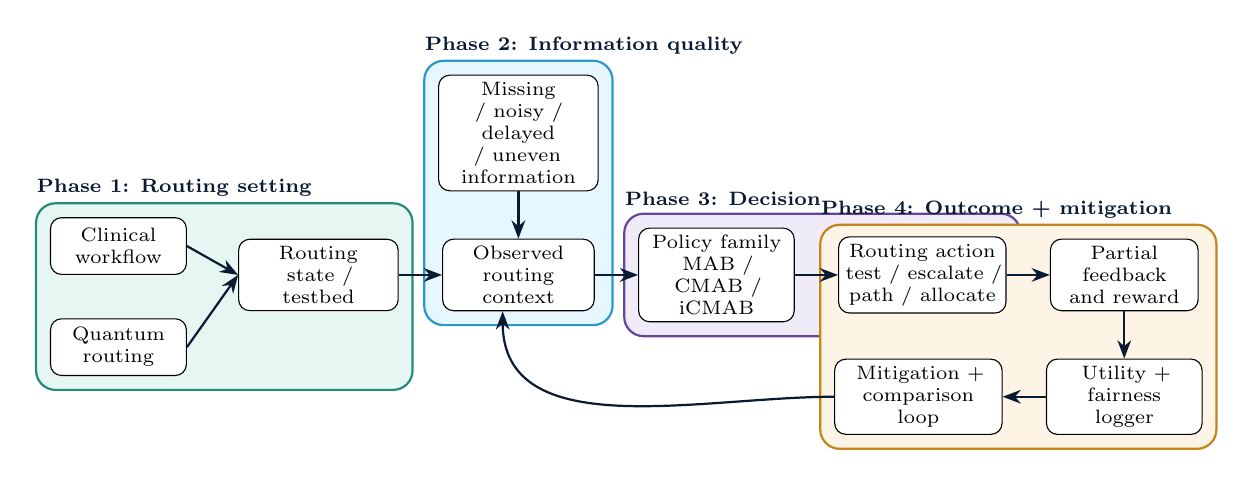
\begin{tikzpicture}[
font=\scriptsize,
box/.style={draw, rounded corners=4pt, align=center, text width=1.55cm, minimum height=0.72cm, inner sep=2.5pt, fill=white},
arr/.style={-Stealth, thick, draw=DeepNavy},
phase/.style={draw, rounded corners=7pt, inner sep=5pt, thick},
phaselabel/.style={font=\scriptsize\bfseries, text=DeepNavy, anchor=west}
]
\node[box] (clin) {Clinical\\workflow};
\node[box, below=0.55cm of clin] (quant) {Quantum\\routing};
\node[box, right=0.65cm of clin.south east, anchor=west, text width=1.85cm] (env) {Routing\\state /\\testbed};
\node[box, right=0.55cm of env, text width=1.75cm] (ctx) {Observed routing\\context};
\node[box, above=0.60cm of ctx, text width=1.85cm] (deg) {Missing / noisy /\\delayed / uneven\\information};
\node[box, right=0.55cm of ctx, text width=1.80cm] (pol) {Policy family\\MAB / CMAB / iCMAB};
\node[box, right=0.55cm of pol, text width=1.95cm] (act) {Routing action\\test / escalate /\\path / allocate};
\node[box, right=0.55cm of act, text width=1.70cm] (fb) {Partial feedback\\and reward};
\node[box, below=0.60cm of fb, text width=1.80cm] (log) {Utility + fairness\\logger};
\node[box, left=0.55cm of log, text width=1.95cm] (mit) {Mitigation +\\comparison loop};

\begin{scope}[on background layer]
\node[phase, fill=PhaseGreen!12, draw=PhaseGreen!80!black, fit=(clin)(quant)(env)] (p1) {};
\node[phase, fill=PhaseBlue!12, draw=PhaseBlue!80!black, fit=(ctx)(deg)] (p2) {};
\node[phase, fill=PhasePurple!12, draw=PhasePurple!80!black, fit=(pol)(act)] (p3) {};
\node[phase, fill=PhaseOrange!12, draw=PhaseOrange!80!black, fit=(fb)(log)(mit)] (p4) {};
\end{scope}

\node[phaselabel] at ([xshift=-0.10cm,yshift=0.18cm]p1.north west) {Phase 1: Routing setting};
\node[phaselabel] at ([xshift=-0.10cm,yshift=0.18cm]p2.north west) {Phase 2: Information quality};
\node[phaselabel] at ([xshift=-0.10cm,yshift=0.18cm]p3.north west) {Phase 3: Decision};
\node[phaselabel] at ([xshift=-0.10cm,yshift=0.18cm]p4.north west) {Phase 4: Outcome + mitigation};

\draw[arr] (clin.east) -- (env.west);
\draw[arr] (quant.east) -- (env.west);
\draw[arr] (env) -- (ctx);
\draw[arr] (deg) -- (ctx);
\draw[arr] (ctx) -- (pol);
\draw[arr] (pol) -- (act);
\draw[arr] (act) -- (fb);
\draw[arr] (fb) -- (log);
\draw[arr] (log) -- (mit);
\draw[arr] (mit.west) to[out=180,in=270] ([xshift=-0.20cm]ctx.south);
\end{tikzpicture}%
}
\par\vspace{0.5em}
\small\textbf{Figure 1.} Color-coded shared domain model. The same four phases support both settings while preserving domain-specific meanings for routing state, action, reward, and fairness metrics.
\label{fig:domain_model}
\end{center}

\end{document}
